\chapter{Testes e Validação}

Este capítulo detalha as estratégias de garantia de qualidade (QA) e as metodologias de validação aplicadas para atestar a integridade, o desempenho e a segurança do ecossistema Poke-Adocao. O processo de homologação afasta-se de validações empíricas manuais em prol de uma esteira de testes automatizados com cobertura arquitetural contínua.

\section{Cenários de Teste e Automação}

A validação do fluxo transacional de ponta a ponta (\textit{End-to-End}) é assegurada por testes unitários e de integração rigorosos, divididos entre os dois pólos do monorrepositório, isolando as responsabilidades de estado e de interface.

\subsection{Validação do \textit{Backend}}
No ambiente de servidor, a infraestrutura de testes é orquestrada pela \textit{framework} \textit{Pytest}, acoplada à extensão \textit{pytest-asyncio} para suportar a resolução do \textit{event loop} do FastAPI. O banco de dados relacional é interceptado, e as transações de teste ocorrem em bases \textit{SQLite} em memória para evitar poluição de dados persistentes.
Os cenários homologados na base de código garantem as invariantes do domínio espacial e transacional:
\begin{itemize}
    \item \textbf{Motor Espacial (\texttt{test\_spatial\_service.py}):} Testes focados em atestar a precisão matemática da Fómula de Haversine e a delimitação dos vértices da \textit{Bounding Box} contra anomalias trigonométricas de latitude e longitude.
    \item \textbf{Máquina de Estados (\texttt{test\_adoption\_service.py}):} Validação da transição unidirecional da \textit{AdoptionStatus}, forçando falhas deliberadas como adoção concorrente da mesma entidade (\textit{race conditions}), violação da distância máxima de 50 metros e excedente do limite de inventário da \textit{party}.
    \item \textbf{Contratos de API (\texttt{test\_api.py} e \texttt{test\_auth.py}):} Verificação da emissão de \textit{tokens} criptográficos, proteção de rotas restritas e sanitização de requisições HTTP malformadas.
\end{itemize}

\subsection{Validação do \textit{Frontend}}
Na camada cliente, a integridade da aplicação móvel \textit{React Native} é aferida através do motor \textit{Jest} e das bibliotecas de dom \textit{React Native Testing Library}.
Os testes isolam o comportamento da interface do usuário da latência de rede:
\begin{itemize}
    \item \textbf{Comportamento de Hooks (\texttt{useUserLocation.test.ts}):} Simulação do ciclo de vida dos sensores do dispositivo móvel para assegurar que a telemetria geográfica é corretamente capturada, filtrada e exposta ao contexto da aplicação.
    \item \textbf{Renderização de Telas (\texttt{LoginScreen}, \texttt{PartyScreen}, \texttt{ProfileScreen}):} Atesta-se a montagem da árvore de componentes, garantindo que o inventário (\textit{Party}) não renderiza instâncias nulas e que o roteamento restringe utilizadores não autenticados.
\end{itemize}

\section{Visão do Usuário}

\begin{figure}[htb]
    \centering
    \caption{Tela de Login}
    \label{fig:login}
    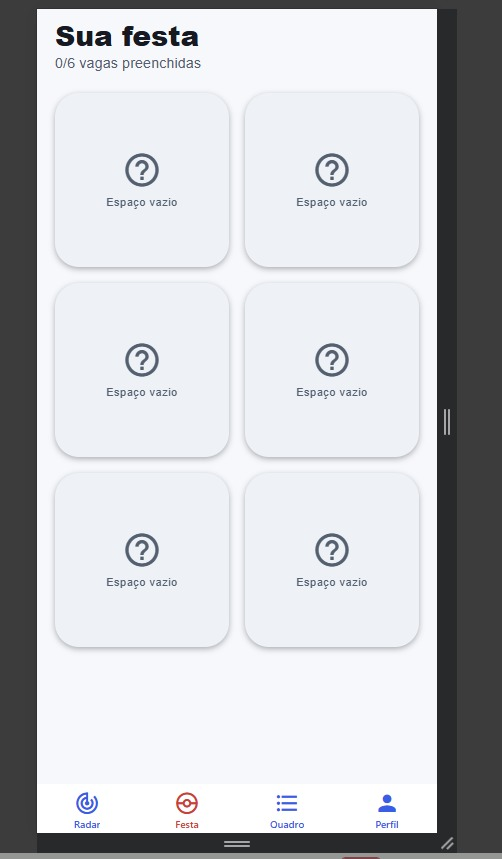
\includegraphics[width=\linewidth, height=0.6\textheight, keepaspectratio]{figure/login.jpeg} 
    \fonte{Elaborado pelos autores (2026).}
\end{figure}

\begin{figure}[htb]
    \centering
    \caption{Tela do grupo de pokemons do usuário (party)}
    \label{fig:party}
    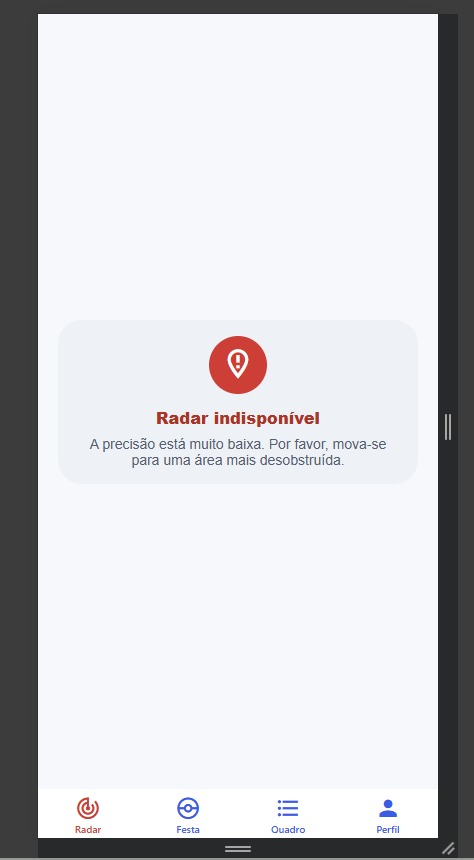
\includegraphics[width=\linewidth, height=0.6\textheight, keepaspectratio]{figure/party.jpeg} 
    \fonte{Elaborado pelos autores (2026).}
\end{figure}

\begin{figure}[htb]
    \centering
    \caption{Tela da lista de adoções vazia}
    \label{fig:lista_de_adocao}
    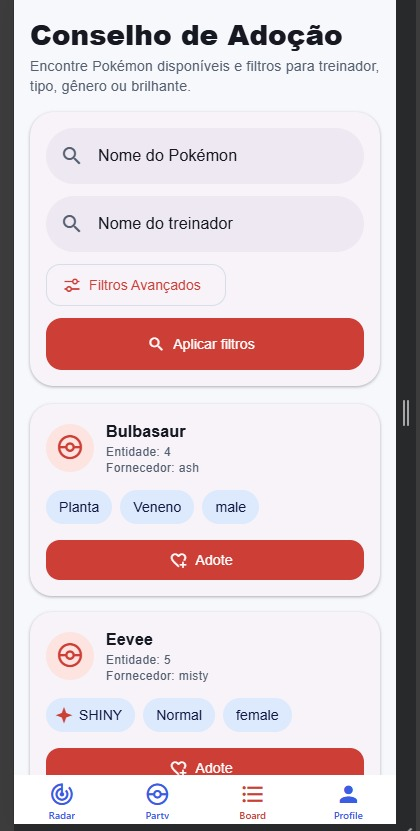
\includegraphics[width=\linewidth, height=0.6\textheight, keepaspectratio]{figure/lista_de_adocao.jpeg} 
    \fonte{Elaborado pelos autores (2026).}
\end{figure}

\begin{figure}[htb]
    \centering
    \caption{Tela da lista de adoções populada}
    \label{fig:lista_de_adocao_populada}
    \includegraphics[width=\linewidth, height=0.6\textheight, keepaspectratio]{figure/populada.jpeg} 
    \fonte{Elaborado pelos autores (2026).}
\end{figure}

\begin{figure}[htb]
    \centering
    \caption{Tela do Radar (Sem Pokemons ou jogadores perto)}
    \label{fig:radar}
    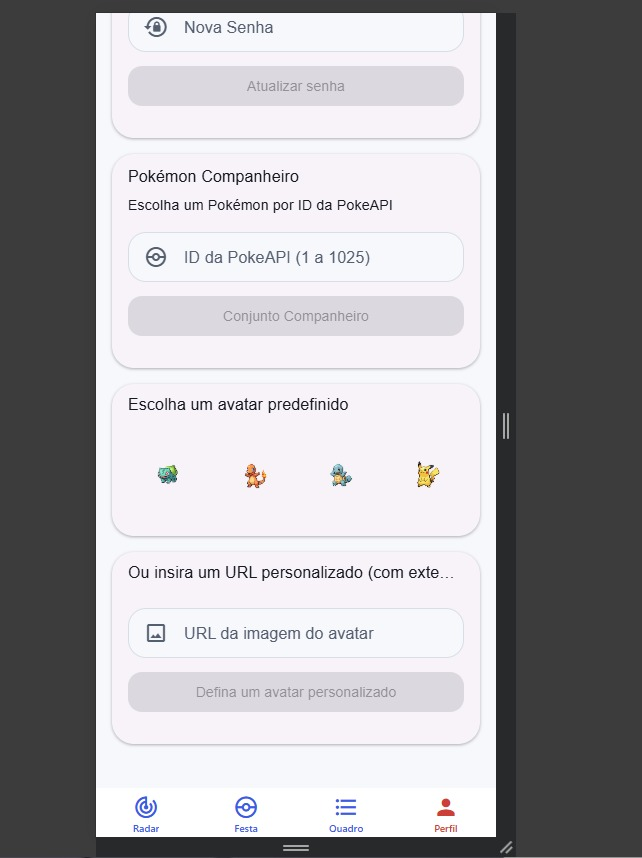
\includegraphics[width=\linewidth, height=0.6\textheight, keepaspectratio]{figure/radar (indisponivel).jpeg} 
    \fonte{Elaborado pelos autores (2026).}
\end{figure}

\begin{figure}[htb]
    \centering
    \caption{Tela do treinador (parte 1)}
    \label{fig:treinadorum}
    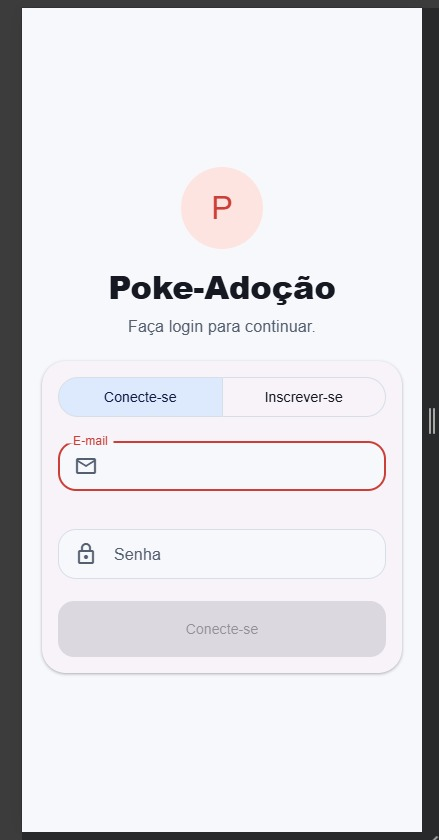
\includegraphics[width=\linewidth, height=0.6\textheight, keepaspectratio]{figure/treinador.jpeg} 
    \fonte{Elaborado pelos autores (2026).}
\end{figure}

\begin{figure}[htb]
    \centering
    \caption{Tela do treinador (parte 2)}
    \label{fig:treinadordois}
    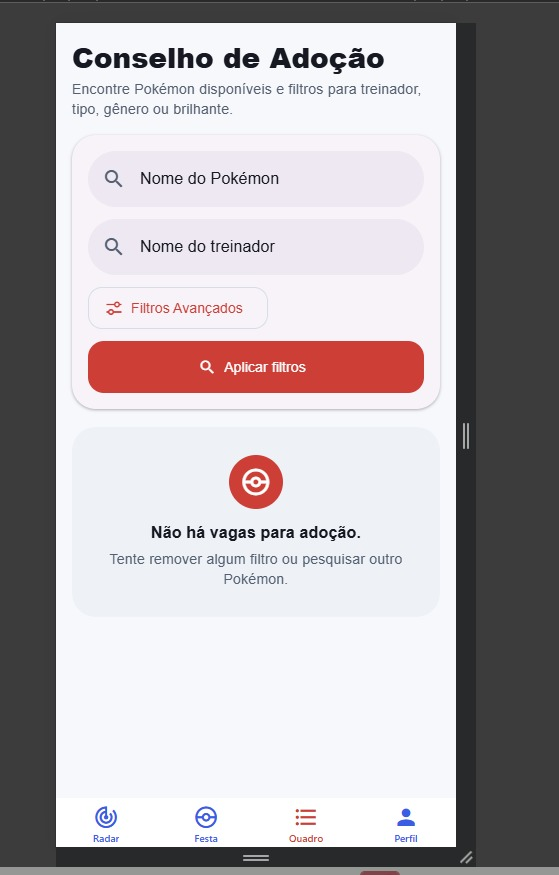
\includegraphics[width=\linewidth, height=0.6\textheight, keepaspectratio]{figure/treinador (final).jpeg} 
    \fonte{Elaborado pelos autores (2026).}
\end{figure}